\section{Emergent Behaviours}

In order to validate the results, we compared the results we obtained against the results presented in the papers by Griffiths and Luck. We consistently found that the donation rate followed the same trends as the original papers, however we noticed that in our implementation the donation rate was higher in all the experiments.

In the following experiments, the donation rate was averaged over 10 runs, each with 1000 generations.

The first test we performed was to test the basic RCA algorithm against the modified one presented in Griffiths 2008. We based our experiments off the same experiments presented in the paper, each of which plot donation rate against: context influence (figure \ref{fig:testing_context_influence}), rewire proportion (figure \ref{fig:testing_rewire_proportion}), population size (figure \ref{fig:testing_population_size}), interaction pairings per generation (figure \ref{fig:testing_interaction_pairings}) and neighbourhood size (figure \ref{fig:testing_neighbourhood_size}).

The donation rate against context influence shows that the donation rate increases with context influence, and closely mirrors the values for donation rate presented in the original paper. These results can be seen in figure \ref{fig:testing_context_influence}.

\begin{figure}[htbp]
	\centering
	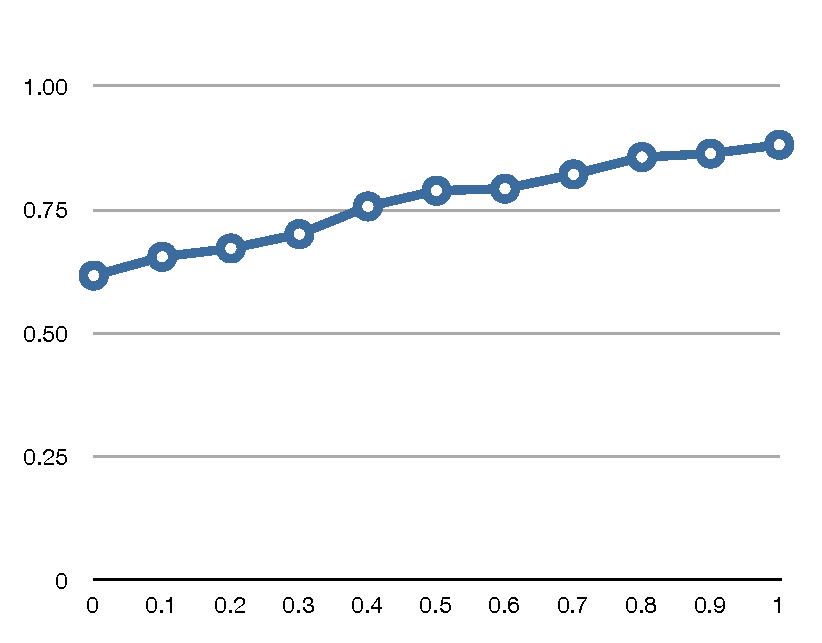
\includegraphics[width=0.4\linewidth]{img/testing_context_influence.pdf}
	\caption{Context Influence against Donation Rate}
	\label{fig:testing_context_influence}
\end{figure}

In a population of 10\% cheaters, the rewire proportion exhibited a similar effect on the donation rate as was presented in the original paper, as shown in figure \ref{fig:testing_rewire_proportion}. It can be seen in the graph that with the random rewire strategy, the rewire proportion has no effect on the donation rate. The random replace worst, individual replace worst and group replace worst exhibit a similar behaviour, when the rewire proportion is 0, the donation rate is the same as the random rewire strategy but when the rewire proportion is increased, the donation rate jumps higher. As presented in the original paper, when the rewire proportion nears 1, the donation rate begins to drop again.

\begin{figure}[htbp]
	\centering
	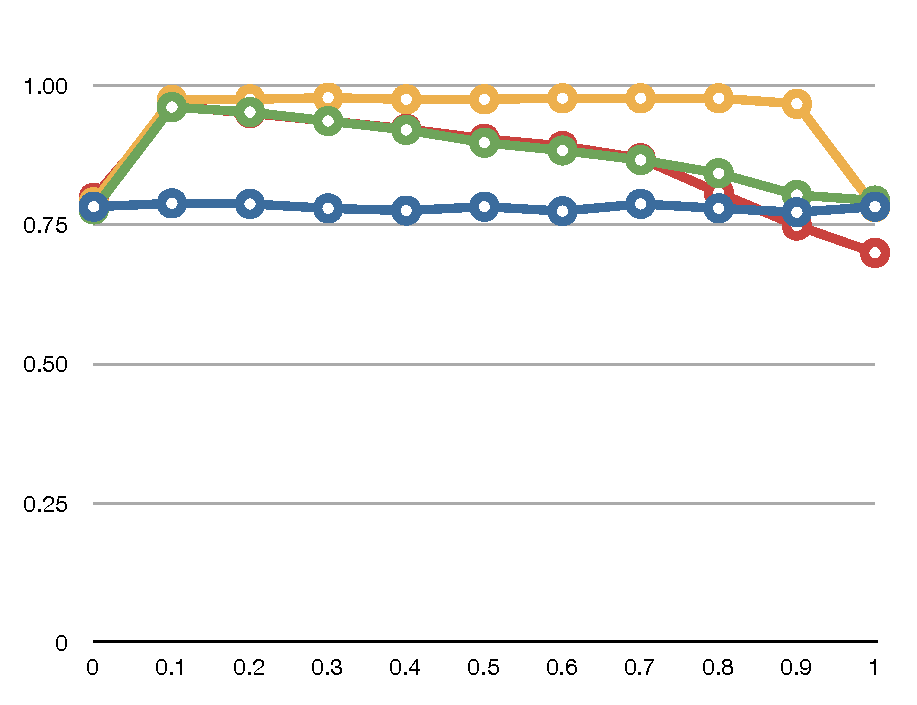
\includegraphics[width=0.4\linewidth]{img/testing_rewire_proportion.pdf}
	\caption{Rewire Proportion against Donation Rate}
	\label{fig:testing_rewire_proportion}
\end{figure}

The graph of population size against donation rate, figure \ref{fig:testing_population_size}, shows that the population size makes no difference to the overall donation rate.

\begin{figure}[htbp]
	\centering
	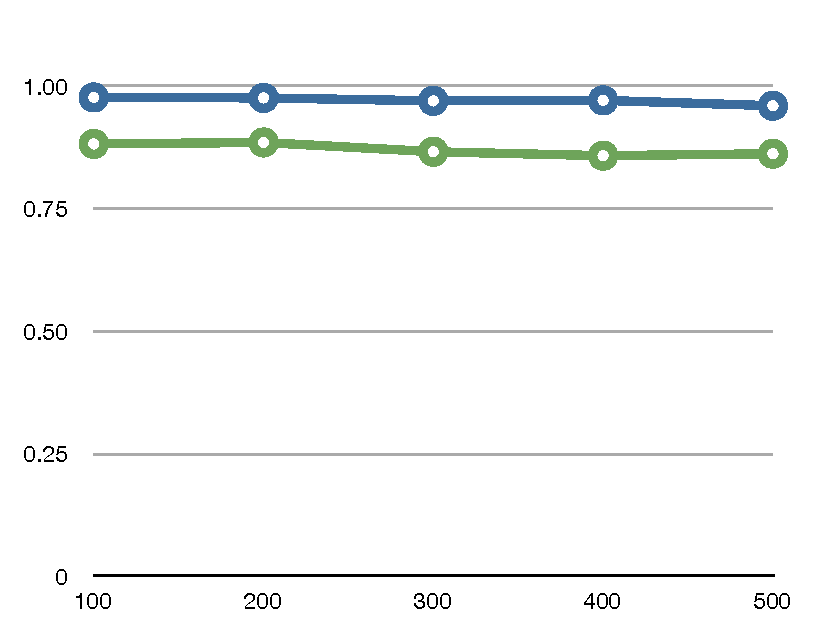
\includegraphics[width=0.4\linewidth]{img/testing_population_size.pdf}
	\caption{Population Size against Donation Rate}
	\label{fig:testing_population_size}
\end{figure}

The number of interaction pairings per generation also has little effect on the donation rate as shown in figure \ref{fig:testing_interaction_pairings}.

\begin{figure}[htbp]
	\centering
	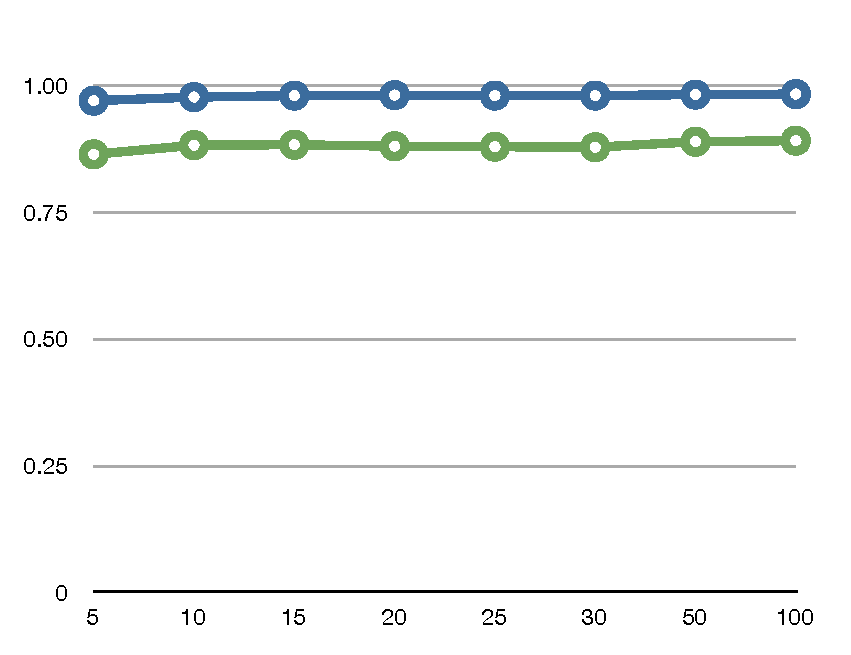
\includegraphics[width=0.4\linewidth]{img/testing_interaction_pairings.pdf}
	\caption{Interaction Pairings against Donation Rate}
	\label{fig:testing_interaction_pairings}
\end{figure}

From the graph that shows the neighbourhood size against donation rate, figure \ref{fig:testing_neighbourhood_size}, it can be seen that the donation rate is fairly similar for small neighbourhoods, but there is a drop in the donation rate when the neighbourhood size reaches 50.

\begin{figure}[htbp]
	\centering
	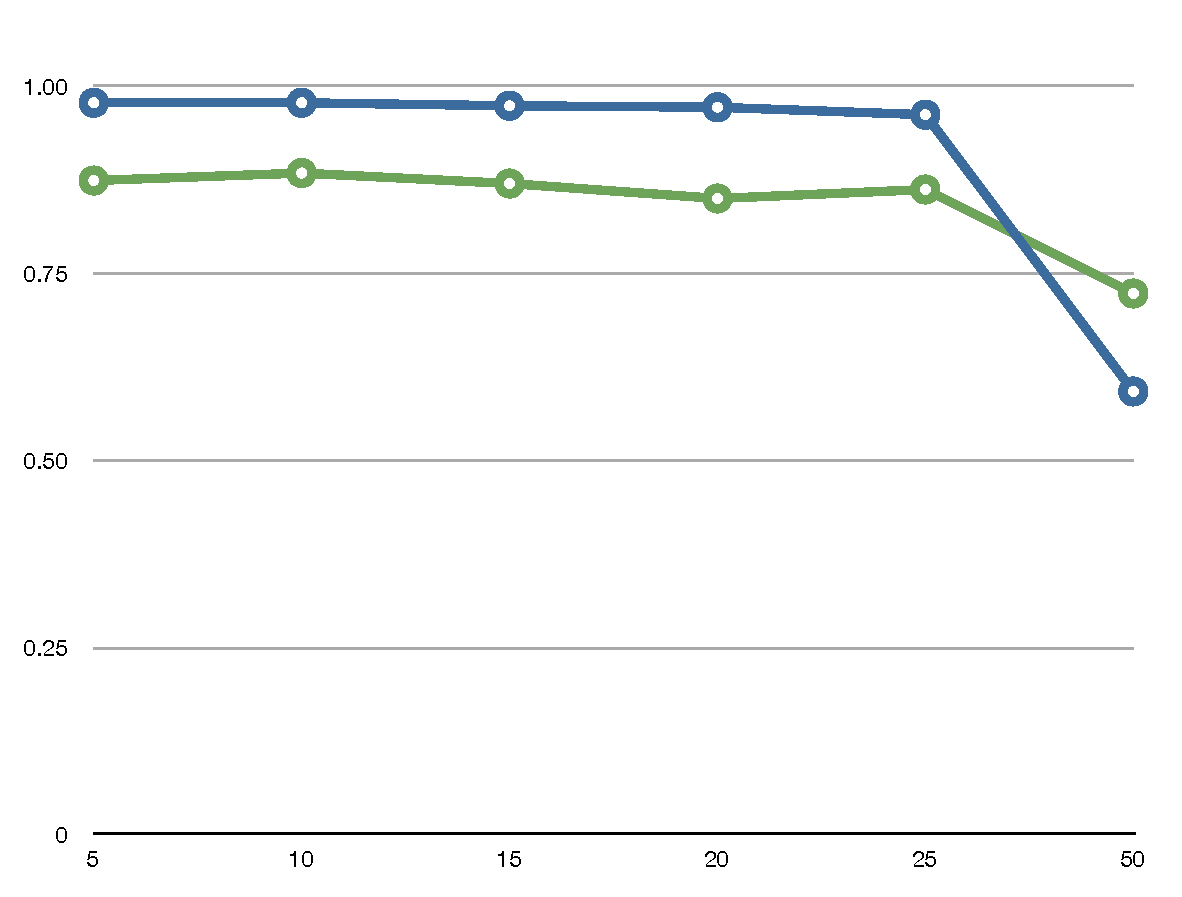
\includegraphics[width=0.4\linewidth]{img/testing_neighbourhood_size.pdf}
	\caption{Neighbourhood Size against Donation Rate}
	\label{fig:testing_neighbourhood_size}
\end{figure}

From these results, we can see that the implementation performs similarly to that of the original papers.